\capitulo{3}{Conceptos teóricos}

El proyecto tiene una relación directa con la minería de datos y los conceptos que lo rodean. 

\section{Minería de datos}

Según IBM \cite{IBM-WhatisDataMining}, podemos definir la minería de datos, o descubrimiento de conocimiento
en los datos \textit{knowledge Discovery in Databases}, como el proceso de descubrir patrones y otra
información a partir de grandes conjuntos de datos. 

Las técnicas de minería de datos principales se pueden dividir en función de sus propósitos principales.
\begin{enumerate}
    \item Descripción del conjunto de datos objetivo.
    \item Predicción de resultados mediante el uso de algoritmos de aprendizaje automático.
\end{enumerate}

\subsection{Proceso de minería de datos}
El proceso seguido en la minería de datos es muy directo. Comienza con la recogida de los datos que van a ser
tratados. y finaliza con la visualización de la información extraída de éstos. 
Los científicos de datos describen los datos a través de sus observaciones de patrones, asociaciones y correlaciones. A su vez se pueden clasificar y agrupar los datos utilizando métodos de clasificación y regresión.

Uno de los marcos de referencia más importantes en el proceso de minado de datos es CRISP-DM, \textit{Cross Industry Standard Process for Data Mining}. Desarrollado por un consorcio de empresas involucradas en la minería de datos. \cite{Chapman2000CRISPDM1S}

\imagen{./img/memoria/CRISP-DM}{Enfoque CRISP de la minería de datos.}

En \cite{KOTU201517} se divide el proceso de la minería de datos en 5 etapas o pasos principales: establecimiento de los objetivos y comprensión del problema, recopilación y preparación de los datos, desarrollo del modelo, aplicación del modelo y la evaluación de los resultados y despliegue en producción.

\begin{enumerate}
   \item \textbf{Establecer los objetivos y comprensión del problema.}
    La primera etapa puede resultar la más complicada del proceso. Todas las partes interesadas deben de estar presentes y de acuerdo en la definición del problema que se va tratar, esto incluye tanto a los científicos de datos como las terceras partes involucradas o interesadas. 
    Este procedimiento ayuda a la formulación de las preguntas de los datos y los parámetros a utilizar en el proyecto. Si se trata de un proyecto empresarial, se debe hacer un estudio o investigación adicional para comprender el contexto de la empresa.
    \item \textbf{Preparación de los datos.}
    Con el alcance del problema definido ya se puede comenzar a identificar qué conjunto de datos será el más efectivo o representativo con el fin de comenzar a dar respuesta a las preguntas formuladas en el proceso anterior.
    
    Una vez se tienen todos los datos recogidos comienza el proceso de pre-procesado de los mismos. Este proceso se basa en la limpieza de los datos con el fin de eliminar cualquier posible ruido, entendiéndose por ruido los datos duplicados, los valores perdidos y aquellos atípicos; aquellos que puedan causar problemas a la resolución del problema o generen incertidumbre.
    En determinados conjuntos de datos se puede hacer una reducción de dimensiones. Consiste en la reducción del número de dimensiones que poseen las instancias recogidas, con el fin de eliminar aquellas que no sean realmente representativas o significativas, este proceso reduce la complejidad de los cálculos posteriores. Por contrapartida hay que conocer cuáles serán los predictores con mayor relevancia en el problema para garantizar una precisión "óptima" del modelo.
    \item \textbf{Desarrollo del modelo.}
    Según \cite{KOTU201517} el modelo es la representación abstracta de los datos y sus relaciones en un conjunto de datos concreto. Actualmente existen cientos de algoritmos que se pueden utilizar, habitualmente proceden de campos como la ciencia de datos, \textit{machine learning}, o la estadística.
    Se debe tener el conocimiento suficiente para entender como funciona el algoritmo para poder configurar correctamente los parámetros que este va a utilizar en base a los datos y el problema de negocio que estamos resolviendo. 
    
    Los modelos en función de como resuelvan el problema que se les presenta se pueden clasificar en:
    \begin{enumerate}
        \item Regresión.
        \item Análisis de asociación.
        \item \textit{Clustering.}
        \item Detección de anomalías.
    \end{enumerate}
    
    El modelo debe ser creado con especial cuidado para evitar el \textit{overfitting}, i.e. el modelo memoriza el conjunto de entrenamiento y no tendrá un rendimiento correcto una vez desplegado en producción. Se desea que el modelo sea lo más generalizado posible de cara a \textit{aprender} de los datos del conjunto de entrenamiento.

    \item \textbf{Aplicación del modelo.}
	El momento de la aplicación del modelo es cuando de verdad se comprueba si realmente el modelo está listo para pasar al siguiente punto, en otras palabras, si es apto para ser desplegado en producción. 
	Para ello se tienen en cuenta métricas como la calidad del modelo ante el problema, su tiempo de respuesta, etc.
    
	\item \textbf{Evaluación de los resultados y despliegue en producción.}
	Una vez que el modelo se encuentra listo es desplegado en producción. Es habitual que los parámetros con los que el modelo fue entrenado con el paso del tiempo dejen de ser los más interesantes, pudiendo ser comprobado el error proporcionado por el modelo con los datos de prueba. Cuando ese error sea excesivo o fuera de un margen dado se deberá de volver a entrenar el modelo, comprobar, y desplegar. 
	De esta forma se puede comprobar como el ciclo de vida del modelo es circular.
\end{enumerate}

El proceso aplicado en la minería de datos proporciona un marco de trabajo mediante el cual se permite extraer información aparentemente no trivial de grandes conjuntos de datos. 
Es un campo de aprendizaje constante, tanto el aplicar los conocimientos del analista para reducir las dimensiones del conjunto de datos, como una vez que se ha entrenado el modelo y puesto en producción aprender los puntos fuertes de este y el porqué de éstos.\cite{Chapman2000CRISPDM1S}

\subsection{Técnicas utilizadas en la minería de datos}
Como se ha comentado anteriormente, uno de los mayores problemas de cara al minado de datos es la dimensionalidad que en muchas ocasiones tienen estos. Es por ello que se aplican técnicas o algoritmos que faciliten la extracción de la información útil. Algunos de ellos son:
\begin{enumerate}
	\item \textbf{Reglas de asociación.} Dado un conjunto de datos concreto, consiste en la aplicación de reglas para encontrar relaciones entre las variables.
	\item \textbf{Redes neuronales.} Principalmente utilizadas en \textit{deep learning}, simulan la interconectividad propia del cerebro humano utilizando capas de nodos. Cada nodo está compuesto por \(x_n\) entradas, \(w_n\) pesos y un sesgo o umbral, el cual al ser superado activa la neurona, pasando los datos del nodo a la siguiente neurona. Habitualmente con una única iteración sobre la red neuronal, esta es capaz de obtener una solución medianamente buena de un conjunto de datos de tamaño considerable. 
	\item \textbf{Árboles de decisión.} Mediante el uso de métodos de clasificación y regresión se clasifican o predicen potenciales resultados en función de un conjunto de decisiones. Utiliza una visualización en forma de árbol para representar los posibles resultados de estas decisiones.
	\item \textbf{k-vecinos más cercanos. KNN (\textit{k-nearest neighbors})} Método no paramétrico de clasificación, sencillo pero eficaz. \cite{hand2007principles} 
Su objetivo es clasificar un conjunto de datos \textit{T}, para ello se recuperan sus \textit{k} vecinos más cercanos, que forman una vecindad de \textit{T}. Se suele utilizar la votación por mayoría entre los registros de datos de la vecindad para decidir la clasificación de \textit{T} con o sin consideración de la ponderación basada en la distancia. \cite{guo2003knn}
\end{enumerate}

\newpage
\section{Aprendizaje en \textit{machine learning}}
En \cite{sanchez_2020} se define \textit{machine learning} como una rama dentro del campo de la Inteligencia Artificial que proporciona a los sistemas la capacidad de aprender y mejorar de manera automática, a partir de la experiencia. Estos sistemas transforman los datos en información, y con esta información pueden tomar decisiones. Este tipo de modelos se crean a base del uso masivo de datos. Cuando se dispone de los datos suficientes para entrenar un modelo comienza el proceso de aprendizaje. El objetivo de este aprendizaje es descubrir patrones ocultos en los datos. En muchas ocasiones el resultado del aprendizaje, el modelo, es una función que dadas unos datos de entrada clasifica o predice correctamente una salida. Como se puede ver en la Figura \ref{fig:../img/memoria/Machine-learning-overview} el aprendizaje automático, \textit{machine learning}, posee diferentes aproximaciones, cada una de ellas con una aproximación diferente en cuanto al uso de instancias etiquetadas.
\imagen{../img/memoria/Machine-learning-overview}{\textit{Machine learning overview}\cite{technovert_2020}}



\subsection{Aprendizaje supervisado}\label{subsec:Aprendizaje-Supervisado}
El aprendizaje automático puede ser resumido como aprender de ejemplos. Al programa se le proporcionan dos conjuntos de datos, uno de entrenamiento y otro de validación.\cite{learned2014introduction} El objetivo es simple, debe de ``aprender'' en función del conjunto de datos etiquetado proporcionado como entrenamiento para posteriormente identificar las correspondientes etiqueta/s de cada instancia del conjunto de validación con la mayor precisión posible. 

Dependiendo del tipo de etiqueta, en el aprendizaje supervisado hay dos modelos.\cite{supervised_learning_mathworks_inc}
\begin{enumerate}
	\item \textbf{Modelos de clasificación.} Producen como salida una etiqueta discreta, i.e. una etiqueta dentro de un conjunto finito de etiquetas, habitualmente suelen ser o binarias $[0,1]$, $[sí,no]$... o multi-etiqueta, donde los valores pueden variar $[0...n]$ (no teniendo porque ser exclusivamente numéricas).

Entre los algoritmos de clasificación más frecuentes encontramos:
	\begin{itemize}
	\item Regresión logística.
	\item \textit{Support Vector Machine, SVM}.
	\item Redes neuronales.
	\item Clasificador Naïve Bayes.
	\item Árbol de decisión.
	\item Análisis discriminante.
	\item K vecinos más cercanos, \textit{KNN}.
	\item Clasificación de ensembles.
	\end{itemize}
	\item \textbf{Modelos de regresión.} Producen como salida un valor real, numérico. Suelen ser soluciones continuas.
	
	Entre los algoritmos de regresión más frecuentes encontramos:
	\begin{itemize}
	\item Regresión lineal.
	\item Regresión no lineal.
	\item Modelo lineal generalizado.
	\item Árbol de decisión.
	\item Redes neuronales.
	\item Regresión con procesos gaussianos.
	\item Regresión con \textit{support vector machines}.
	\item Regresión con ensembles.
	\end{itemize}
	
\end{enumerate}

\subsection{Aprendizaje no supervisado}\label{subsec:Aprendizaje-No-Supervisado}
En la Sección \ref{subsec:Aprendizaje-Supervisado} se comenta que, los modelos para que ``aprendan'' los patrones que se encuentran en los conjuntos de datos, necesitan tener un conjunto de datos etiquetado correctamente para extraer la información de ese conjunto. Pero en los problemas del mundo real no siempre se tienen infinidad de datos disponibles etiquetados correctamente, o simplemente es un proceso muy laborioso y costoso económicamente.

Para solventar este problema se cuenta con el aprendizaje no supervisado\cite{bengio2012unsupervised}, mediante esta técnica no es necesario proporcionar al modelo datos etiquetados. Por definición, el algoritmo encargado de entrenar el modelo  ``aprenderá'' los datos sin conocimiento previo. Para ello el modelo se basará en los datos que tiene disponibles y en la codificación del algoritmo para descubrir los patrones que se encuentren en los datos.

Debido a la forma de trabajar del aprendizaje no supervisado, desde el primer momento en el que el algoritmo tiene los datos comienza a reportar salidas, describiendo la información y categorizando lo que encuentra en los datos.

Principalmente existen dos técnicas de aprendizaje no supervisado.
\begin{enumerate}
	\item \textbf{\textit{Clustering}.}\cite{unsupervised_learning_clustering} Proceso por el cual se dividen los datos no clasificado en grupos aparentemente similares. Cuando se identifican datos con algún parecido entre sí, son agrupados. Permite clasificar e identificar atributos únicos de los datos con los que clasificarlos. 
	
	Un proceso habitual de agrupamiento es el uso de \textit{K-means}, $K\in\mathbb{R}$, donde se indica en $K$ cuántos \textit{clusters} o grupos se han de hacer con los datos. 
	
	Con los datos agrupados el proceso de análisis de éstos puede comenzar. En ocasiones si el número de grupos detectados es muy alto, se pueden encontrar grupos o \textit{clusters} irrelevantes, permitiendo a los científicos de datos eliminar esos datos que los forman, reduciendo la dimensionalidad. 
	
	\item \textbf{Reducción de la dimensionalidad.} La clasificación en el aprendizaje automático se basa en atributos o características que tienen los datos, permitiendo su clasificación, valga la redundancia. Cuando los conjuntos de datos poseen múltiples características, más difícil resulta su clasificación. Es por ello que resulta útil identificar aquellos atributos que están fuertemente interrelacinados entre sí para eliminar todos menos un atributo, reduciendo la dimensionalidad.\cite{li2002unsupervised}
\end{enumerate}

\subsection{Aprendizaje semi-supervisado}\label{subsec:Aprendizaje-Semi-Supervisado}
\textit{Semi-Supervised Learning} según \cite{zhou2014semi}, se define como una forma de entrenamiento de modelos el cual usa tanto datos etiquetados como no etiquetados, i.e. si no sería un aprendizaje supervisado, Sección \ref{subsec:Aprendizaje-Supervisado}, o no supervisado, Sección \ref{subsec:Aprendizaje-No-Supervisado}. 

El uso de aprendizaje semi-supervisado se caracteriza por ser más barato que el supervisado, ya que este último necesita que todo el conjunto de datos que va a utilizar para aprender esté etiquetado, y ese proceso es largo y costoso.Además, obtiene mejores resultados en menor tiempo que el aprendizaje no supervisado. 
Conseguir datos sin etiquetar es una tarea muy sencilla, mientras que conseguir conjuntos de datos etiquetados es un proceso complejo y actualmente no hay ``de todo''.

Para que el aprendizaje sea fructuoso requiere que las instancias se encuentren inter-relacionadas entre sí por alguna de sus características. \cite{javatpoint_semisupervised} indica las siguientes suposiciones que se dan en el aprendizaje semi-supervisado.
\begin{enumerate}
	\item \textbf{Continuidad.} Se asume que los objetos cercanos entre sí se encontrarán en el mismo \textit{cluster} o grupo --- de etiquetas. 
	\item \textbf{\textit{Clustering.}} Las instancias son divididas en diferentes grupos discretos, compartiendo todos los elementos de un \textit{cluster} la misma etiqueta.
	\item \textbf{\textit{Manifold}} o colectores. Se emplea el uso de distancias y funciones de densidad de forma que las instancias se encuentran en colectores con menos dimensiones que el espacio de entrada.
\end{enumerate}

Dentro de las \textit{best preactices} en \textit{semi-supervised learning} se encuentran el uso de diferentes modelos de redes neuronales para el entrenamiento.  \cite{thekumparampil2018attention}
\newpage

\section{Técnicas de selección de instancias}\label{sec:tecnicas-seleccion-instancias}
Dentro de los conjuntos de datos nos encontramos con las instancias, son cada uno de los elementos que componen el \textit{dataset}; en problemas reales de \textit{machine learning} es habitual que se requiera de clasificación automática de estos datos. Este proceso se puede llevar a cabo con algoritmos de aprendizaje supervisado, Sección \ref{subsec:Aprendizaje-Supervisado}, con el objetivo de etiquetar la nueva información. Para poder hacerlo previamente se ha tenido que entrenado el clasificador con un conjunto de entrenamiento, $T$. \cite{olvera2010review}

En la práctica, cualquier $T$ dado contendrá información útil e información desechable, este último tipo de información --- que en realidad son instancias --- a parte de ser redundantes producen ruido, pudiendo inducir en una clasificación errónea en el proceso de aprendizaje, y posteriormente tener un modelo que no sea capaz de clasificar correctamente la nueva información.

\begin{figure}
\centering
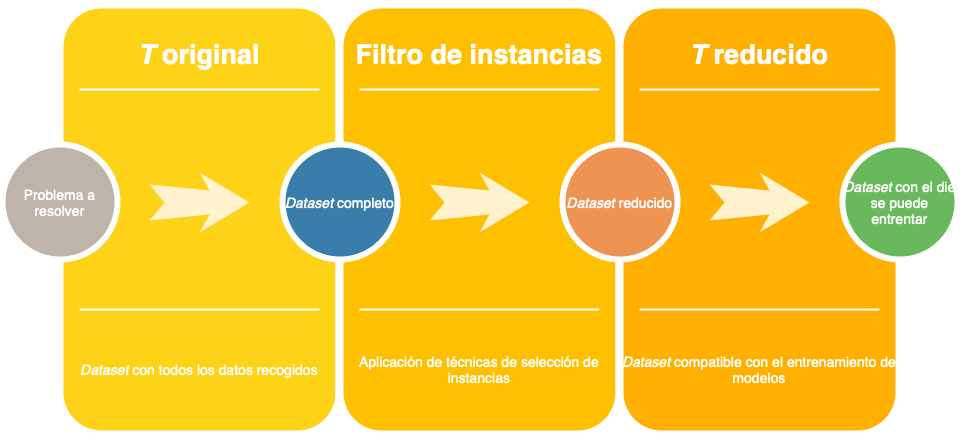
\includegraphics[width=\linewidth]{../img/memoria/Instance-Selection-Overview}
\caption{Proceso de selección de instancias.}
\label{fig:instance-election-overview}
\end{figure}

Es por ello que un pre-procesado o \textbf{filtrado} de las instancias pertenecientes al $T$ original es necesario. En la Figura \ref{fig:instance-election-overview} se puede consultar de manera gráfica el proceso de selección de instancias. Dado un conjunto de datos de entrenamiento inicial, $T$, el objetivo será obtener un subconjunto $S$, tal que $S \subseteq T$ de manera que $S$ no contiene instancias redundantes ni ``ruidosas''. Además, $Acc(S) \cong Acc(T)$, donde $Acc(X)$ es la precisión, \textit{accuracy} en inglés, del modelo entrenado con el conjunto de datos $X$.

En función de cómo comienzan a crear el nuevo subconjunto de datos, $S$, se identifican dos aproximaciones, ascendente y descendente.
\begin{itemize}
\item \textbf{Ascendente.} El nuevo conjunto de datos comienza estando vacío, $S = \emptyset$, y a medida que se vayan realizando iteraciones del algoritmo correspondiente, se irán añadiendo instancias a $S$. El principal problema que posee esta aproximación es su sensibilidad al orden, i.e. dada una instancia $x \subset T$, en diferentes iteraciones del mismo algoritmo de selección de instancias sobre el mismo $T$, puede o no estar en $S$. Esto se debe a la aleatoriedad con la que se presentan los datos, para asegurar esta aleatoriedad los datos se escogen de manera aleatoria de $T$, intrínsecamente da una mayor facilidad a las muestras iniciales a estar en $S$ que las finales, ya que puede que ya se encuentren representadas o sean clasificadas como ruido.

Entre las principales ventajas de esta aproximación destaca el espacio de almacenamiento requerido, puesto que se van guardando instancias y por lo tanto en un inicio es muy pequeño.

\item \textbf{Descendente.} El nuevo conjunto de datos comienza siendo el conjunto de entrenamiento al completo, $S = T$, y a medida que se vayan realizando las iteraciones del algoritmo correspondiente, se irán eliminando instancias de $S$. Esta aproximación es mucho más costosa computacionalmente, para cada instancia que debe decidir si eliminar o no debe comprobar todo el subconjunto $S$, pero en contraposición consigue reducir más que la aproximación ascendente, el conjunto de entrenamiento $T$.
\end{itemize}

Junto con esta diferenciación, en función de la aproximación de selección de instancias existen dos agrupaciones.
\begin{itemize}
\item \textbf{\textit{Wrapper}.} El criterio de selección se basa en la precisión del clasificador. Aquellas instancias que no contribuyen a la mejora del clasificador se quedan fuera de $S$. Este trabajo está centrado en este criterio de selección.
\item \textbf{\textit{Filter}.} El criterio de selección utiliza una función, $f(x, y)$, para realizar la selección, no se basa en el clasificador.
\end{itemize}

\begin{table}[]
\begin{center}
	\begin{tabular}{@{}ccc@{}}
	\toprule
	\rowcolor[HTML]{EFEFEF} 
	\textbf{Método} & \textbf{Basado en}       & \textbf{Referencia} \\ \midrule
	ENN             & Clasificación incorrecta & \cite{wilson1972asymptotic}\\ \midrule
	\rowcolor[HTML]{EFEFEF} 
	CNN             & Clasificación incorrecta & \cite{hart1968condensed}\\ \midrule
	RNN             & Clasificación incorrecta & \cite{gates1972reduced}  \\ \midrule
	\rowcolor[HTML]{EFEFEF} 
	ICF             & Alcance y covertura      & \cite{brighton2002advances}\\ \midrule
	MSS             & Fronteras de decisión    & \cite{barandela2005decision}\\ \bottomrule
	\end{tabular}
\end{center}
\caption{Algunos métodos de selección de instancias.}
\label{tab:instance-selection-methods}
\end{table}

En la Tabla \ref{tab:instance-selection-methods} se aprecian aquellos algoritmos implementados en primera instancia para la reducción de instancias dentro de $T$, el objetivo de todos ellos es que el subconjunto generado, $S$, sea capaz de clasificar correctamente  $T$ en su totalidad prácticamente.

\section{Algoritmos de selección de instancias}
Existen multitud de algoritmos a día de hoy que son capaces de reducir el número de instancias de $T$, en este trabajo se van a comentar los pertenecientes a la Tabla \ref{tab:instance-selection-methods}. Cada uno de ellos tiene sus ventajas y sus desventajas como cabe esperar, en la literatura no apreciamos un ``este es mejor que aquel'' o similar.

\subsection{Algoritmo de edición de Wilson}
Wilson \cite{wilson1972asymptotic} (1972) publicó la regla del vecino más cercano editado, \textit{ENN}. Los problemas de clasificación de instancias en función de una etiqueta, se caracterizan por:
\begin{itemize}
\item Hay una instancia a ser clasificada.
\item Existe un $S$ el cual posee instancias con la misma distribución que la instancia a clasificar, pudiendo ser comparables las instancias del conjunto con la que estamos analizando.
\item No existe información adicional del conjunto.
\item Existe una distancia medible entre instancias.
\end{itemize}

Con todas estas premisas Wilson propone un algoritmo basado en clasificación incorrecta en función de sus vecinos más cercanos. Cuando una instancia resulta mal clasificada por sus \textit{k} vecinos más cercanos, \textit{k}-NN, esa instancia es descartada. Finalmente obtendremos como resultado un conjunto $S$ con las instancias correctamente clasificadas por sus vecinos.

Suponiendo que sea \textit{X} un conjunto de \textit{N} instancias y \textit{M} posibles clases y, sea \textit{k} el número de vecinos cercanos,el algoritmo de Wilson se puede formular de la siguiente manera:

\begin{algorithm}
\caption{Algoritmo de edición de Wilson, \textit{ENN}.}\label{alg:Wilson-ENN}
\begin{algorithmic}[1]
\Require Conjunto de entrenamiento, $X=\left\{(x_1,y_1)...(x_n,y_n)\right\}$, $k$ vecinos.
\Ensure Conjunto editado $S \subset X$.
\Statex
\Procedure{ENN}{$X, k$}
	\State $S=X$
	\ForAll{$x \in S$}
		\State Find x.$N_{1...k+1}$, the $k+1$ nearest neighbors of $x \in X - \{x\}$
		\If{$\delta_{k-NN}\left(x_i\right)\not=\theta_i$}
			\State Remove $x$ of $S$
		\EndIf
	\EndFor
	\State return $S$
\EndProcedure
\end{algorithmic}
\end{algorithm}

El algoritmo de edición de Wilson, ver Algoritmo \ref{alg:Wilson-ENN} posee una complejidad computacional de $O(n^2)$. Una de las ventajas de este algoritmo es su forma de crear el subconjunto $S$, ya que al ser descendente las primeras iteraciones serán lentas --- dependiendo del tamaño de $T$ lógicamente --- pero las finales serán considerablemente más rápidas.

\newpage
\section{Función distancia entre instancias}
La función distancia proporciona la proximidad entre dos instancias en función de todos sus parámetros. Si la distancia que separa dos instancias es cero, ambas instancias son idénticas. Se tiende a trabajar con conjuntos de datos normalizados, i.e. todos los datos son ajustados a una escala común, independientemente de la escala en la que hayan sido medidos.

Existen multitud de métricas para calcular la distancia, pudiendo variar la distancia calculada en función de cuál se aplique. Se van a comentar las más representativas.
\begin{itemize}
\item \textbf{Distancia de Minkowski.} La distancia de Minkowski es una métrica en el espacio vectorial normalizado. Es una métrica que se puede modificar con facilidad para calcular la distancia entre dos instancias de diferentes maneras. 
\begin{enumerate}
\item \(p = 1\), cálculo de la distancia de Manhattan.
\item \(p = 2\), cálculo de la distancia Euclídea.
\item \(p = \infty\), cálculo de la distancia de Chebyshov.
\end{enumerate}
Su fórmula es la siguiente:
\[ \mathbb{D}(x, y) = \left( \sum_{i=1}^{n}\left| x_i - y_i \right|^p \right)^{1/p} \]

\item \textbf{Distancia de Manhattan} o distancia del taxista. Es una métrica en un espacio vectorial normalizado, calculándose como la suma de los $n$ segmentos verticales u horizontales que unen dos puntos.

Su fórmula es la siguiente:
\[  \mathbb{D}(x, y) = \sum_{i=1}^{d}\left| x_i - y_i\right| \]

\item \textbf{Distancia euclidiana} o norma L2 o distancia L2. Es la distancia en línea recta entre dos puntos de datos en el espacio euclidiano.

Su fórmula normalizada es la siguiente:
\[  \mathbb{D}(x, y) = \sqrt{\sum_{i=1}^{d} \frac{\left(x_i - y_i\right)^2}{\sigma_i^2}}  \]

\item \textbf{Distancia de Chebyshow} o distancia del tablero de ajedrez. La distancia entre dos puntos es la mayor de sus diferencias a lo largo de cualquiera de sus dimensiones coordenadas.

Su fórmula es la siguiente:
\[  \mathbb{D}(x, y) = \max_i\left(\left|x_i - y_i\right|\right) \]

\item \textbf{Distancia del Coseno.} Mide la similitud o distancia entre dos vectores calculando el coseno del ángulo que forman.

Su fórmula es la siguiente:
\[ \mathbb{D}(x, y) = \frac{\sum_{i=1}^{d}x_iy_i}{\sqrt{\sum_{i=1}^{d}x_i^2}\sqrt{\sum_{i=1}^{d}y_i^2} } \]

\item \textbf{Distribución de Pearson} o $\chi^2$. 

\end{itemize}
\newpage
